\documentclass[11pt, oneside]{article}   	% use "amsart" instead of "article" for AMSLaTeX format
\usepackage{geometry}                		% See geometry.pdf to learn the layout options. There are lots.
\geometry{letterpaper}                   		% ... or a4paper or a5paper or ... 
%\geometry{landscape}                		% Activate for rotated page geometry
%\usepackage[parfill]{parskip}    		% Activate to begin paragraphs with an empty line rather than an indent
\usepackage{graphicx}				% Use pdf, png, jpg, or eps§ with pdflatex; use eps in DVI mode
								% TeX will automatically convert eps --> pdf in pdflatex	
\usepackage{amssymb}
\usepackage[tbtags]{amsmath}
\usepackage{tikz}
\usepackage{pgfplots}
\pgfplotsset{width=6cm,compat=1.9}
\usepackage[toc,page]{appendix}
\usepackage{graphicx}
\graphicspath{ {images/} }

\title{An FMM for the Modal Green's Function}
\date{May 4, 2016}

\begin{document}
\maketitle

\section{Introduction}
This project examines the problem of constructing of a fast multipole method (FMM) algorithm for an important category of non-uniform density distributions: axisymmetric surfaces of revolution.
%This project examines the problem of constructing of a fast multipole method (FMM) algorithm for density distributions on axisymmetric surfaces of revolution using the symmetry of the surface to represent the kernel as the modal Green's function.

We will work in three-dimensional cylindrical coordinates $(r,\theta,z)$ such that a point in Cartesian coordinates $(x,y,z)$ is represented by:
\begin{align*}
x &= r\cos\theta\\
y &= r\sin\theta\\
z &= z
\end{align*}

An axisymmetric, or rotationally symmetric, surface $\Gamma$ is one that has symmetry along the $\theta$-axis. The surface $\Gamma$ is obtained by rotating a two-dimensional curve $\gamma$ about the $z$ axis. $\gamma$ is called the generating curve. In particular, $\Gamma=\gamma\times\mathbb{T}$ where $\mathbb{T}$ is the one-dimensional torus (circle) parametrized by $\theta\in(-\pi,\pi]$.
\begin{center}
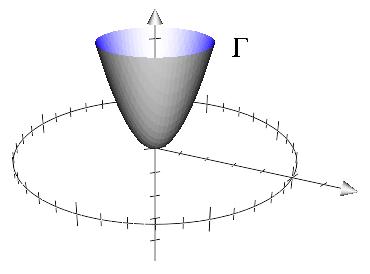
\includegraphics[scale=0.5]{bowl3}
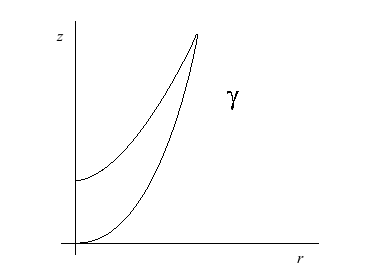
\includegraphics[scale=0.5]{bowl}
\end{center}
% HIGHLIGHT
Describe the need for a modal FMM, or FMM for axisymmetric surfaces with difficult geometries. This need stems from the number of discretization points needed to accurately represent complicated generating curves. For example, a circular generating curve is easy to discretize with some finite number of points equally spaced, however for a rectangle, we need more discretization points in the corners. Finally, for something like a thin strip with a circle, we need many many discretization points in this small space. The problem of many sources distributed in close proximity, or clumping.
\begin{center}
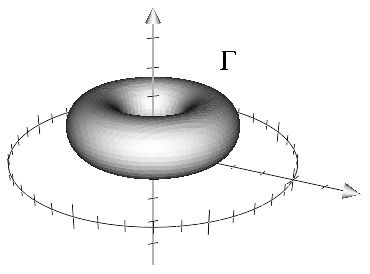
\includegraphics[scale=0.5]{torus}
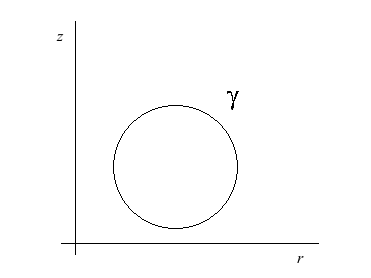
\includegraphics[scale=0.5]{circle}
\end{center}
\begin{center}
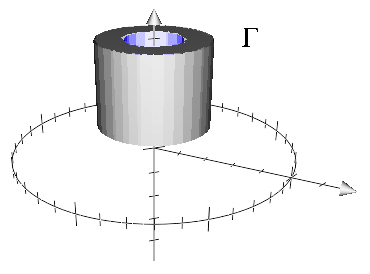
\includegraphics[scale=0.5]{pipe2}
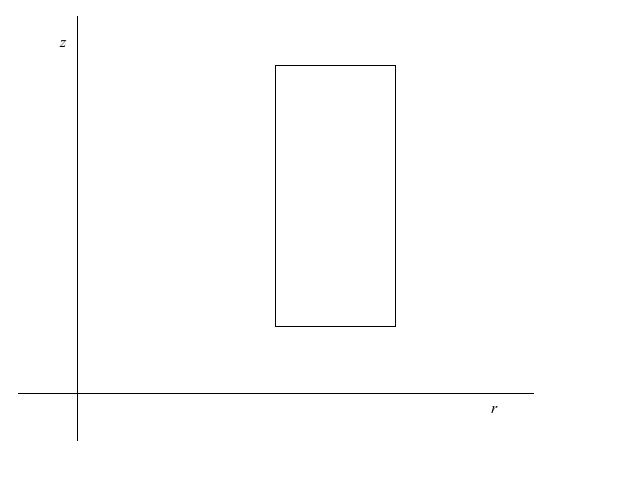
\includegraphics[scale=0.5]{rect}
\end{center}
Density distributions on axisymmetric surfaces have many applications. The problem of electromagnetic scattering by a surface of revolution has radar, geophysical exploration, and acoustics applications. This type of problem relies precisely on creating a fast algorithm for an axisymmetric density distribution.

\section{Statement of problem}
Consider $N$ source points $\mathbf{y}_j=(r'_j,\theta'_j,z'_j)$ distributed on this surface $\Gamma$, with each assigned a charge $\sigma_j$. We want to compute the potential $f$ at target points $\mathbf{x}_i=(r_i,\theta_i,z_i)$ also on $\Gamma$ due to the source densities.  In practice, the same set of points act as both sources and targets. The potential is represented by the sum
\begin{align}
f(\mathbf{x}_i) = \sum_{j=1}^N K(\mathbf{x}_i,\mathbf{y}_j)\sigma_j
\end{align}
where $K(\mathbf{x},\mathbf{y})$ is a kernel, typically the Green's function of the partial differential equation that describes the potential between two points in the domain. In particular, we are interested in the free-space (without boundary conditions) Green's function for Laplace's equation:
\begin{align}
K(\mathbf{x},\mathbf{y}) = \frac{1}{4\pi |\mathbf{x}-\mathbf{y}|}
\end{align}
%This is specifically for charges governed by a Dirichlet problem with Laplace's equation. On a three-dimensional surface $\Gamma$,
%\begin{align}
%\Delta u &= 0 \mbox{ in }\Omega\\
%u &= f \mbox{ on }\Gamma
%\end{align}
The goal is to construct a fast summation method for equation $(1)$ that takes advantage of the rotational symmetry of $\Gamma$.

\section{Modal Green's Function}

The crucial technique to construct a fast method for an axisymmetric density distribution is to reduce the problem in three dimensions to a series of problems in two dimensions using Fourier analysis. In $\S3.1$, we should the derivation of this Fourier representation for an arbitrary kernel, then for the Green's function f Laplace's equation. The efficacy of this strategy is grounded in the fact that it is easier to solve boundary integral equations defined on curves in $\mathbb{R}^2$ than those defined on surfaces in $\mathbb{R}^3$.

We are able to reduce the problem in this way because the rotationally symmetric nature of $\Gamma$ yields $K(\mathbf{x},\mathbf{y})$ symmetric along the $\theta$-axis such that the kernel is a function of the difference $\theta-\theta'$:
\begin{align*}
K(\mathbf{x},\mathbf{y})=K(\theta-\theta',r,z,r',z')
\end{align*}
We call such a kernel rotationally invariant.

Recall that if for two any points $\mathbf{x}$ and $\mathbf{y}$ in the computational domain a kernel can be written
\begin{align*}
K(\mathbf{x},\mathbf{y}) = K(|\mathbf{x}-\mathbf{y}|)
\end{align*}
then it is called translation invariant. Notice that the Green's function for Laplace's equation is translation invariant. Not all kernels are translation invariant, however, and the fact that what we'll define in $\S3.1$ as the modal Green's function is not translation invariant is crucial to the difficulty of creating an optimal FMM in this scenario.

\subsection{Fourier representation of 3D integral equations}
This follows closely \cite{YYM}.
Consider the Fredholm integral equation of the first kind defined on $\Gamma$:
\begin{align}
f(\mathbf{x}) &= \int_\Gamma K(\mathbf{x},\mathbf{y})\sigma(\mathbf{y})d\mathbf{y} &\mathbf{x},\mathbf{y}\in\Gamma
\end{align}
This is a 3D integral equation, essentially a continuous version of equation $(1)$, which can just be viewed as a discretization of this integral equation.

We can represent $(3)$ as a sequence of 2D integral equations defined on the generating curve $\gamma$ by performing Fourier transformations on $f$, $\sigma$, and $K$.. If $f_m$, $\sigma_m$, and $k_m$ are the Fourier modes of $f$, $\sigma$, and $K$, respectively, then we have
\begin{align*}
f_m(r,z)&=\int_\mathbb{T}\frac{e^{-im\theta}}{\sqrt{2\pi}}f(r,z,\theta)d\theta&f(\mathbf{x})&=\sum_{m\in\mathbb{Z}}\frac{e^{im\theta}}{\sqrt{2\pi}}f_m(r,z)\\
\sigma_m(r,z)&=\int_\mathbb{T}\frac{e^{-im\theta}}{\sqrt{2\pi}}\sigma(r,z,\theta)d\theta&\sigma(\mathbf{x})&=\sum_{m\in\mathbb{Z}}\frac{e^{im\theta}}{\sqrt{2\pi}}\sigma_m(r,z)\\
k_m(r,z,r',z')&=\int_\mathbb{T}\frac{e^{-im\theta}}{\sqrt{2\pi}}K(r,z,r',z',\theta)d\theta&K(\mathbf{x},\mathbf{y})&=\sum_{m\in\mathbb{Z}}\frac{e^{im(\theta-\theta')}}{\sqrt{2\pi}}k_m(r,z,r',z')
\end{align*}
such that
\begin{align}
\sqrt{2\pi}\int_\gamma k_m(r,z,r',z')\sigma_m(r',z')r'dl(r',z')&=f_m(r,z) &(r,z),(r',z')\in\gamma
\end{align}
for each $m\in\mathbb{Z}$.

In practice, we choose a truncation parameter, $M\in\mathbb{N}$, such that $f$ is well-represented by its lowest $2M+1$ Fourier modes
\begin{align}
||f-\sum\limits_{m=-M}^{M}\frac{e^{in\theta}}{\sqrt{2\pi}}f_m||\le\epsilon
\end{align}
and only compute the lowest $2M+1$ Fourier modes for each of the functions $f$, $\sigma$, and $K$.

We are using the Green's function of a PDE as our kernel, so $k_m$ is called the modal Green's function. In particular, we are interested in the Fourier expansion of the Green's function for Laplace's equation
\begin{align}
\frac{1}{4\pi |\mathbf{x}-\mathbf{y}|} &=\frac{1}{4\pi\sqrt{r^2+r'^2-2rr'\cos{(\theta-\theta')}+(z-z')^2}}\\
&= \sum_{m\in\mathbb{Z}} \frac{e^{im(\theta-\theta')}}{\sqrt{2\pi}} s_m(r,z,r',z')
\end{align}
where the modal Green's function is
\begin{align}
s_m(r,z,r',z')=\frac{1}{\sqrt{8\pi^3 rr'}}\mathbf{Q}_{m-\frac{1}{2}}\bigg(\frac{r^2+(r')^2+(z-z')^2}{2rr'}\bigg)
\end{align}
with $Q_{m-\frac{1}{2}}$ the half-integer order Legendre function of the second kind. Notice that while $K$ was translation invariant, $s_m$ is not. This has implications which we discuss later.

Now rather than constructing a fast summation for a density distribution on $\Gamma$ using $K(\mathbf{x},\mathbf{y})$, we can construct a series of fast summations for a density distribution on $\gamma$ using $s_m(r,z,r',z')$.

We should note that for now we are only considering the Green's function for Laplace's equation because its Fourier modes can be solved for analytically. For many other kernels, it is not possible to find the same type of explicit formula, and we would need to approximate the modes using a discretization as in \cite{YYM}.

We should also note that for densities distributed on the axisymmetric surface $\Gamma$ the computational domain was a subset of $\mathbb{R}^3$. For the densities distributed on $\gamma$, however, we only need to consider the right half-plane of $\mathbb{R}^2$ as the computational domain.

In the next sections, we give an overview of the FMM, and discuss how several well-known fast methods approach the problem of axisymmetric density distributions.

\section{The fast multipole method}
FMMs are insensitive to density distribution unlike FFT. it is a fast approximation algorithm, with higher complexity yielding higher accuracy.

Explain more about the sum being computed...this is the naive sum...this is what it represents.

The FMM was developed initially by Greengard and Rokhlin as a way to accelerate the computation of potential between points as in equation $(1)$. In general, it reduces the complexity of matrix-vector multiplication from $\mathcal{O}(N^2)$ to $\mathcal{O}(N)$ or $\mathcal{O}(N\log N)$ for a given error level $\epsilon$. They did this using a multipole expansion for the Green's function of a system such that sources clumped together could be viewed as a single source to a far-field target.

1. generation of a hierarchical tree partitioning of the computational domain;
2. accumulation of the multipole expansions for the far field by a postorder traversal of the tree;
3. translation of the multipole moments to the local expansions;
4. construction of local expansions by a preorder traversal of the tree;
5. evaluation of the far-field action on the particles using local expansions;
6. evaluation of the near field interactions.

TALK ABOUT INTERACTION LIST

For two dimensions, the single-layer Laplacian kernel is $K(\mathbf{x},\mathbf{y})=-\frac{1}{2\pi}\log(|\mathbf{x}-\mathbf{y})$. It is convenient, however, to write $K(\mathbf{x},\mathbf{y})=Re(\log(z_x-z_y))$ where $z_x$ and $z_y$ are complex number corresponding to points $\mathbf{x}$ and $\mathbf{y}$ in the plane. The idea of FMM is to encode the potentials of a set of source densities using the multipole expansion and local expansion at places far away from these sources. Suppose the source densities are supported in a disk centered at $z_C$ with radius $r$. Then for all z outside the disk with radius $R (R > r)$, we can represent the potential at $z$ from the source densities using a set of coefficients $\{a_k ; 0 \le k \le p\}$, where
\begin{align}
f(z)=a_0\log(z-z_C)+\sum_{k=1}^p\frac{a_k}{(z-z_C)^k}+\mathcal{O}\bigg(\frac{r^p}{R^p}\bigg)
\end{align}

On the other hand, if the source densities are outside the disk with radius $R$, the potential at a point $z$ inside the disk with radius $r$ can be represented using a set of coefficients $\{c_k, 0\le k\le p\}$, where
\begin{align}
f(z)=\sum_{k=0}^pc_k(z-z_C)^k+\mathcal{O}\bigg(\frac{r^p}{R^p}\bigg)
\end{align}

In both expansions, $p$ is usually a small constant determined by the desired accuracy of the result. 

The FMM employs these expansions recursively. The computational domain, a box containing all source and target points, is hierarchically partitioned into a tree structure (a quadtree in 2D or an octtree in 3D). Each node of the tree corresponds to geometric box (square or cube). The tree is constructed so that the leaves contain no more than a prespecified number of points. For each box, the potential induced by its source densities is represented using a multipole expansion, while the potential induced by the sources from non-adjacent boxes is encoded in a local expansion.

Not only these expansions (multipole and local) can be used for efficient evaluation, but translations between these expansions are also available which make an $\mathcal{O}(N)$ algorithm possible. In particular, the following types of translations are used:

M2M The multipole to multipole translation transforms the multipole expansions of a bchildren to its own multipole expansion.

M2L. The multipole to local translation transforms the multipole expansion of a box to the local expansion
of another non-adjacent box.

L2L. Finally, the local to local translation of the local expansion of a boxparent to its own local expansion.

See Appendix B for the equations that define these translations.

Using the tree structure, FMM consists of two basic steps. During the first step, the upward pass, the tree
is traversed in postorder 4 to compute the multipole expansion for each box. At the leaves, the multipole
expansions are built following Eq. (1) (this procedure is also called the source to multipole (S2M) translation).
At each non-leaf node, the multipole expansion is shifted from its children using the M2M
translation. In the second step, the downwards pass, the tree is traversed in a preorder 5 to compute the local
expansion. For each box B, the local expansion is the sum of two parts: first, the local-to-local transformation
collects the local expansion of B parent (the result condenses the contributions from the sources in
all the boxes which are not adjacent to Bparent), and second, the multipole-to-local transformation
collects the multipole expansions of the boxes which are the children of the neighbors of Bparent but are
not adjacent to B (these boxes compose the interaction list of B). The sum of these two parts encodes all the
contribution from the sources in the boxes which are not adjacent to B itself. At the end, for each box, the
far interaction, which is evaluated using the local expansion at this box (this step is called the local to target
(L2T) translation), is combined with the near interaction evaluated by iterating over all the source points in
the neighborhood of the target box to obtain the potential (see Fig. 1).
Instead of Laurent series, in three dimensions the far field is represented by spherical harmonics. There
are several implementation details (mostly for the M2L transformation) that are required for efficient
implementation (especially in 3D), but we do not mention them here. Overall, however, the organization of
the computation is the same as the two dimension case. For the derivation of the expansions and a detailed
discussion on error bounds and implementation details see [7,14].

\subsection{The full algorithm}
\begin{enumerate}
\item Populate a computational domain with source and target points.
\item Partition the computational using a quadtree of boxes with levels $0,\dots,L$ until each box contains no more than $s$ source points.
\item UPWARD PASS: -For each box on the finest level, construct a multipole expansion. - translate the multipole expansions to the parent box for each level
\item DOWNWARD PASS: - beginning with the coarsest level with an interaction list (level $2$), construct a local expansion for each box.
\end{enumerate}

\subsection{Analysis-based FMMs}

(special functions FMM)

The classical FMM \cite{GR} first developed by Greengard and Rokhlin relies on analytic expansions for the potential. The multipole expansion for a box is the potential at some target in the far field due to sources in the box. The local expansion for a box is the potential at a target in the box due to all sources in the far field. They used Legendre polynomials and spherical harmonics to represent the kernel $1/\mathbf{r}$.
\begin{align}
\frac{1}{|\mathbf{x}-\mathbf{y}|} = \sum
\end{align}

The three-dimensional problem is currently not possible as stated with an analytic FMM since we do not yet have multipole or local expansions for the Green's function for Laplace's equation in three-dimensional cylindrical coordinates.

We can consider an analytic FMM for the series of modal Green's functions, but again the analytic expansion has not been determined, and in fact, may not even exist. Our attempts to construct such expansions have so far failed. The necessary analytic machinery for the kernels $s_n$ does not exist yet if at all, and is in fact, very inefficient to construct. In addition, this method will require the evaluation of special functions. This is costly.

\subsection{Kernel-Independent Methods}

linear algebraic and PDE(green's idnentities)

Since we don't have the analytic machinery required for an analysis-based FMM, we consider kernel-independent methods. These methods don't require the same analytic expansions, and instead use equivalent densities to represent the source densities. These methods can be separated into two categories. First, the not so kernel-independent methods which require that the kernel is the Green's function for some elliptic partial differential equation, or satisfies Green's identity. The most well-known method of this type is the kernel-independent FMM (KIFMM), which was proposed by Ying, Biros, and Zorin. Second are methods which work with any smooth kernel and require only its evaluation at some points. The most well-known method of this type is the black-box FMM (bbFMM) by Fong and Darve.

%In the first type of method, we want to use the properties of the PDE to construct translation operators. There are three approaches we can use to represent the potential in the far-field: 1) use Green's third identity -- differential equations, 2) use integral equations, or 3) create equivalent densities and potentials. 3) is the choice of YBZ, and further detail of the construction of these operators is explored below. Essentially, an algorithm of this type depends on the source to multipole translation, and choice of a discretization scheme.

\subsection{Translation Operators}
In the analysis-based FMM, a translation operator translates a multipole or local expansion of one box to that of another in the computational domain. In kernel-independent methods, translation operators translate equivalent densities in the same way. Translation operators are the backbone of a fast multipole algorithm because these operations are how we reduce the number of direct computations required to compute the sum in equation $(1)$. Translation operators can be computed without any knowledge of the source or target points, so they are a true pre-computation. The only thing required is a computational domain and choice of a number of level.

EXPAND TO FULL ALGORITHM
There are five different translation operators. The source-to-multipole (S2M) operator creates a multipole expansion for a given box. The multipole-to-multipole (M2M) operator translates densities in a box to densities in its parent box. The multipole-to-local (M2L) operator translates densities in a box to another box on the same level in the hierarchical tree that divides the computational domain. The local-to-local (L2L) operator translates densities in a box to densities in a child box. Lastly, the local-to-target (L2T) operator computes the far field interaction for the target points using the local expansion.

If a kernel is translation invariant, then translation operators will only differ based on relative position and level in the hierarchical tree. This is due to the the kernel's dependence only on the difference between coordinate values, e.g. $(|\mathbf{x}-\mathbf{y}|)$. For example, with a translation invariant kernel the $M2L$ operation from the box $[0,1]\times[0,1]$ to $[0,1]\times[2,3]$ would be the same as the operation from $[1,2]\times[1,2]$ to $[1,2]\times[3,4]$. Therefore many translation operators on a given level are identical, and need not be computed repeatedly. In fact, each level has at most $40$ $(7^2-3^2)$ unique transfer vectors.

On the other hand, if a kernel is not translation invariant, then every translation operator for every box in the computational domain needs to be computed. Every transfer vector is unique, so none can be reused or recycled as above. This is the case for the modal Green's function, and we need to take this more costly pre-computation into consideration when evaluating a fast method.

\section{The KIFMM}
Rather than using analytic multipole and local expansions like in the FMM, the KIFMM substitutes a continuous distribution of upward and downward equivalent densities that lie on surfaces surrounding each box in the hierarchical tree to represent the potential generated by sources in that box and the potential in that box due to sources in the far-field. To find this equivalent density, we match its potential to the potential of the original sources at a surface, in the far field, by solving local Dirichlet-type boundary value problems.EXPLAIN EQUIVALENT DENSITIES BETTER. In this algorithm the equivalent of a multipole expansion is the potential at a far-field target due to an equivalent density lying on an equivalent surface surrounding the box of sources. The equivalent of a local expansion is the potential at a target due to the equivalent densities of all far-field source boxes. This allows us to construct an efficient FMM that only requires kernel evaluations. This method relies on Green's third identity. The idea is that for well-separated boxes (at least one box away), the actual naively-computed potential between sources and targets in these boxes is the same as the potential due to these equivalent densities. The target box can't tell the difference between the real source densities and the equivalent densities. One advantage of the KIFMM is that it is relatively easy to implement, since in general it applies to an arbitrary kernel that is the fundamental solution of some elliptic PDE. To change the kernel in the original FMM, one would need to develop analytic multipole and local expansions, which as aforementioned are difficult to find if they exist at all, and the requirement of special functions makes them inefficient to construct.

To avoid the difficulty required in the implementation of the 3D KIFMM, the technique of using the modal Green's functions described earlier and covered at length by Yao, Young, and Martinsson, in \cite{YYM} is used -- replacing the 3D integral equations required by the 3D KIFMM with their Fourier representations, sequences of 2D integral equations. In this way, the 3D KIFMM implementation is avoided in favor of repeatedly applying the 2D KIFMM. As mentioned earlier, this strategy is currently only applicable to the modal Green's function for Laplace's equation because we can analytically determine its Fourier modes.

One downside to this application is that the pre-computation of translation operators is not optimal due to the not translation invariant kernel. In an attempt to reduce this pre-computation, we tried to find constant proportionality between the operators. For example, we consider that perhaps the $M2L$ from $[0,1]\times[0,1]$ to $[2,3]\times[0,1]$ is in proportion to the translation from $[0,1]\times[0,1]$ to $[3,4]\times[0,1]$. However, these attempts failed and indeed since the translation operators in the KIFMM are simply kernel evaluations, we wouldn't expect this relationship to exist because it doesn't hold for the not translation invariant kernel. So every translation operator for every box on every level would need to be pre-computed. This is computationally expensive because every operator involves the evaluation of the kernel.

It's important to note that since the translation operators rely on kernel evaluations, they will also differ for each mode of the Fourier expansion of the Green's function since we're essentially using a different kernel. That means the full algorithm will require the pre-computation of $2M+1$ times the number of operators required for the computational domain, where $M$ is the truncation parameter for the Fourier expansion. Another consequence of the kernel reliance for translation operators is the added cost due to the fact that these translations will depend on which mode of the Fourier expansion we are using. Essentially, the entire FMM process would need to be done separately $2M+1$ times. This is in sharp contrast to the computational savings of the vectorization of this process that's possible in the black-box FMM, which we discuss next.

\section{The black-box FMM}
The black-box FMM is a Chebyshev interpolation-based $\mathcal{O}(N)$ algorithm for non-oscillatory kernels. In general, this algorithm uses equivalent densities in each box placed at Chebyshev nodes. In this section, we consider this scheme to quickly compute this sum for each modal Green's function
\begin{align}
f_m(\mathbf{x}_i)=\sum_{j=1}^N s_m(\mathbf{x}_i,\mathbf{y}_j)\sigma_{m,j}
\end{align}
for targets $\mathbf{x}_i$ and sources $\mathbf{y}_j$.

The bbFMM is good for complicated analytic kernels. Unlike the FMM or KIFMM, it requires only a smooth kernel, and only uses kernel evaluations at specific points. Another advantage for this method is that it has a small pre-computation even for large systems. The pre-computation for any kernel is $\mathcal{O}(N)$. This is a crucial advantage for the bbFMM in this problem since the pre-computation for the KIFMM varied based on the kernel evaluations and so was expensive because of the not translation invariant kernel. Another important advantage for the bbFMM is that only the $M2L$ operation requires an evaluation of the kernel. This means that the other four operations do not change based on which mode of the Fourier expansion of the Green's function, so they need not be computed separately for each mode.

The full method combines the methods of SVD compression from...
\begin{align}
s_m(\mathbf{x},\mathbf{y})=\sum_i \alpha_i u_i(\mathbf{x})v_i(\mathbf{y})
\end{align}

and Chebyshev interpolation as in....
\begin{align}
s_m(\mathbf{x},\mathbf{y})=\sum_i\sum_j s_m(\mathbf{x}_i,\mathbf{y}_j)w_i(\mathbf{x})w_j(\mathbf{y})
\end{align}

First we need to define the $n$th Chebyshev polynomial
\begin{align}
T_n(x)=\cos\bigg(n\arccos\bigg(\frac{2}{b-a}\bigg(x-\frac{a+b}{2}\bigg)\bigg)\bigg)
\end{align}
on $[a,b]$. The Chebyshev nodes, which are the $n$ roots of the Chebyshev polynomial, on $[a,b]$ are
\begin{align}
x=\frac{a+b}{2}+\frac{b-a}{2}\cos\bigg(\frac{2i-1}{2n}\pi\bigg)\mbox{ for }i=1,\dots,n.
\end{align}
in one dimension. For two dimensions, there are $n^2$ Chebyshev nodes that are the tensor product of the Chebyshev nodes of each interval on the two axes $r$ and $z$. The nodes in the box these intervals create are all of the possible $(r,z)$ pairs of the nodes in each respective interval, making $n^2$ nodes in each box.

From the Chebyshev polynomial Fong and Darve derive the optimal (why?) interpolation functions
\begin{align}
R_n(\mathbf{x},\mathbf{y}) = \bigg(\frac{1}{n} + \frac{2}{n}\sum_{i=1}^{n-1}T_n(r)T_n(z)\bigg)\bigg(\frac{1}{n} + \frac{2}{n}\sum_{i=1}^{n-1}T_n(r')T_n(z')\bigg)
\end{align}
for $\mathbf{x}=(r,z)$ and $\mathbf{y}=(r',z')$.

From there we use a low-rank approximation for the $m$th modal Green's function given by
\begin{align}
s_m(\mathbf{x},\mathbf{y}) = \sum_{l_1=1}^n\sum_{l_2=1}^n\sum_{m_1=1}^n\sum_{m_2=1}^n s_m(\mathbf{\overline{x}}_{l_1,l_2},\mathbf{\overline{y}}_{m_1,m_2})R_n(\mathbf{\overline{x}}_{l_1,l_2},\mathbf{x})R_n(\mathbf{\overline{y}}_{m_1,m_2},\mathbf{y})
\end{align}
to approximate the sum
\begin{align}
f_m(\mathbf{x}_i)=\sum_{l_1=1}^n \sum_{l_2=1}^n R_n(\mathbf{\overline{x}}_{l_1,l_2},\mathbf{x}_i) \sum_{m_1=1}^n \sum_{m_2=1}^n s_m(\mathbf{\overline{x}}_{l_1,l_2},\mathbf{\overline{y}}_{m_1,m_2}) \sum_{j=1}^N \sigma_{m,j}R_n(\mathbf{\overline{y}}_{m_1,m_2},\mathbf{y}_j)
\end{align}
where $N$ is the number of source points, $n^2$ is the number of Chebyshev nodes in each box, $\mathbf{y}_j$ are the source points, $\mathbf{x}_i$ are the target points, $\mathbf{\overline{x}}_{l_1,l_2}$ are the Chebyshev nodes in the target box, and $\mathbf{\overline{y}}_{m_1,m_2}$ are the Chebyshev nodes in the source box.

This low-rank approximation yields the translation operators for this method. For a given mode $n=m$, we detail each operation.
\subsection{S2M}
The source-to-multipole operation computes weights $W^{m,B}_{m_1,m_2}$ at each Chebyshev node $\mathbf{\overline{y}}_{m_1,m_2}$ by anterpolation in a box $B$ on the finest level.
\begin{align}
W_{m_1,m_2}^{m,B} = \sum_{\mathbf{y}_j\in B} \sigma_{m,j} R_n(\mathbf{\overline{y}}^B_{m_1,m_2},\mathbf{\overline{y}}_j)
\end{align}
for $m_1,m_2 = 1,\dots,n$.
\subsection{M2M}
The multipole-to-multipole operation translates weights at the nodes of four child boxes $B_i$, $W_{m_1,m_2}^{m,B_i}$, to weights at the nodes of its parent box $A$, $W_{m_1,m_2}^{m,A}$.
\begin{align}
W_{m_1,m_2}^{m,A} = \sum_{i=1}^4 \sum_{m'_1=1}^n\sum_{m'_2=1}^n W_{m'_1,m'_2}^{m,B_i} R_n(\mathbf{\overline{y}}^A_{m_1,m_2},\mathbf{\overline{y}}^{B_i}_{m'_1,m'_2})
\end{align}
for $m_1,m_2= 1,\dots,n$.
\subsection{M2L}
The multipole-to-local operation computes the far-field contribution at Chebyshev nodes $\mathbf{\overline{x}}_{l_1,l_2}^A$ in box $A$ from all boxes $B_i$ in the interaction list of $A$.
\begin{align}
g_{l_1,l_2}^{m,A} = \sum_{B_i} \sum_{m_1=1}^n\sum_{m_2=1}^n W_{m_1,m_2}^{m,B_i} s_m(\mathbf{\overline{x}}^{A}_{l_1,l_2},\mathbf{\overline{y}}^{B_i}_{m_1,m_2})
\end{align}
for $l_1,l_2 = 1,\dots,n$.
\subsection{L2L}
On the root level let $f^{m,A}_{l_1,l_2}=g^{m,A}_{l_1,l_2}$ and use the local-to-local operation to obtain the full local expansion by adding the far-field contribution from the parent box $B$
\begin{align}
f^{m,A}_{l_1,l_2}=g^{m,A}_{l_1,l_2} + \sum_{l'_1=1}^n \sum_{l'_2=1}^n f^{m,B}_{l_1,l_2} R_n(\mathbf{\overline{x}}_{l_1,l_2}^A,\mathbf{\overline{x}}_{l'_1,l'_2}^B)
\end{align}
for $l_1,l_2 = 1,\dots,n$ where $B$ is the parent box of box $A$.
\subsection{L2T}
The local-to-target operation computes $f_m(\mathbf{x}_i)$ for target point $\mathbf{x}_i$ in box $B$ by interpolating the far-field approximation.
\begin{align}
f_m(\mathbf{x}_i)=\sum_{l_1=1}^n \sum_{l_2=1}^n f^{m,B}_{l_1,l_2} R_n(\mathbf{\overline{x}}_{l_1,l_2}^B,\mathbf{x}_i)
\end{align}

Notice that the $S2M$, $M2M$, $L2L$, and $L2T$ translation operators in this scenario do not require kernel evaluations. Since the interpolation functions $R_n$ do not depend on which mode of the Fourier representation of the Green's function, we only need to compute these operators once instead of $2M+1$ times in the KIFMM.

In addition, for each mode $m$, the weights $W^{m,B}_{m_1,m_2}$ can be represented by a matrix with $n^2$ rows and $M$, the truncation parameter discussed earlier chosen for the Fourier representation, columns. Therefore these translation operations are just matrix-matrix multiplications which can be performed quickly in practice.

%HIGHLIGHT
\subsection{Vectorization}
Vectorization of the bbFMM for modal Green's function. A key advantage of this method over the KIFMM is the fast pre-computation and indeed fast application of these operators. Not only can they all be computed at once since the interpolation function does not depend on the Fourier mode $m$, but the operators can be applied quickly as well. To see this, consider that $\sigma_{m,j}$ is an $N\times (2M+1)$ matrix, where each row is the source point and each column is a Fourier mode, which we can apply via BLAS3 matrix-matrix multiplication to the interpolation function $R_n$. $W_{m_1,m_2}^{m,B}$, too, is then simply a matrix for each box with rows representing each Chebyshev node and each column representing a Fourier mode. We can now do all of these operations for EVERY MODE at once! This is a huge advantage over the KIFMM where we would need to separately complete the entire pre-computation and application process $2M+1$ times for each node.
\\

$W^m=R_n \sigma_m$\\

$W_{all} = R_n \sigma_{all}$\\

The $M2L$ operation deserves a little special attention since it does depend on the kernel $s_m$ and is the most expensive pre-computation and operation. The computation of $s_m$, however, generates each of the $2M+1$ Fourier modes all at once using the Fast Fourier Transform (FFT).

\begin{align}
s_m = \int_0^{2\pi} \frac{1}{4\pi|\mathbf{x}-\mathbf{y}|}e^{-im\theta'}d\theta'
\end{align}

for x far from y, use discrete FFT on |x-y| to get $s_m$ for M2L. for x near y, use Johan Helsing or Martinsson and Miller's algorithm to compute $Q_{m-1/2}$, $Q_{m+1/2}$, $Q_{m+3/2}$, etc.

As previously mentioned, the evaluation of $s_m$ at the Chebyshev nodes can be accelerated using any of the techniques described in \cite{A}, \cite{VBT}, and \cite{YFC}. The efficient evaluation of modal Green's function for Laplace's equation, and the $Q$-function in particular, has been explored. The methods described there can be implemented to quickly evaluate $s_m$.

The full bbFMM also reduces the cost of the $M2L$ operation by using SVD compression. However, with a not translation invariant kernel some of these operations may not save anything since recyclable transfer vectors on each level was crucial to their argument.

\section{Future Work}
Complete the bbFMM algorithm for modal Green's function.

\begin{appendices}
\section{Legend}
\begin{align*}
&N \mbox{ the number of source points in the computational domain}\\
&m \mbox{ the index for each Fourier mode of the Green's function}\\
&M \mbox{ the truncation parameter for the Fourier expansion of the Green's function}\\
&n \mbox{ the number of Chebyshev nodes in each interval}\\
&\mathbf{x}_i\mbox{ target points}\\
&\mathbf{\overline{x}}_{l_1,l_2}\mbox{ Chebyshev nodes in the target box}\\
&\mathbf{y}_j\mbox{ source points}\\
&\mathbf{\overline{y}}_{m_1,m_2}\mbox{ Chebyshev nodes in the source box}\\
\end{align*}


\section{Implementation and Testing}
Currently, we are able to produce and have tested all equivalent densities and translation operators with Python programs for the Chebyshev interpolation-based bbFMM. However, for now we are just using the kernel, $\log|\mathbf{x}-\mathbf{y}|$, instead of the modal Green's function for Laplace's equation. These functions are very similar, though, so we expect these tests to succeed with the modal Green's function as well.

Much of the future work to do is a full FMM implementation in Python. Key pieces of this will be accelerating the $M2L$ operation by efficiently evaluating the modal Green's function, using the vectorization discussed in $\S6$, and using singular value decomposition (SVD) compression technique described in \cite{CGMR}, \cite{FD}, \cite{ZGR} and \cite{MV}.

The following are descriptions of the computations done by each of our test programs.\\
$\mathbf{2D-S2M.py}$
\begin{enumerate}
\item Put $N$ sources in box $A$ and assign charges of $\pm 1$.
\item Put target in a box $B$ in the far field.
\item For each Chebyshev node of $A$, assign a weight\\
$$W_{m_1,m_2}=\sum_{j=1}^N \sigma_j R_n(\mathbf{\overline{y}}_{m_1,m_2},\mathbf{y}_j)$$
\item Compute the potential at each Chebyshev node in a target box $B$\\
$$f_{l_1,l_2}=\sum_{m_1=1}^n\sum_{m_2=1}^n W_{m_1,m_2} \log(\mathbf{\overline{x}}_{l_1,l_2},\mathbf{\overline{y}}_{m_1,m_2})$$
\item Compute the potential at the target by interpolation\\
$$f(\mathbf{x}_i)=\sum_{l_1=1}^n\sum_{l_2=1}^n f_{l_1,l_2} R_n(\mathbf{\overline{x}}_{l_1,l_2},\mathbf{x}_i)$$
\item Compare the result with the naive computation of the potential\\
$$f(\mathbf{x}_i)=\sum_{j=1}^N \log(\mathbf{x}_i,\mathbf{y}_j) \sigma_j$$
\end{enumerate}

$\mathbf{2D-M2M}$
\begin{enumerate}
\item Put $N$ sources in box $A$ and assign charges of $\pm 1$.
\item For each Chebyshev node of $A$, assign a weight\\
$$W_{m_1,m_2}=\sum_{j=1}^N \sigma_jR_k(\mathbf{\overline{y}}_{m_1,m_2},\mathbf{y}_j)$$
\item Repeat step $2$ for the four child boxes $B_i$ of $A$. Note that there will be $\le N$ sources in each child box.
\item Use the $M2M$ operation to compute\\
$$W^A_{m_1,m_2}= \sum_{i=1}^4\sum_{m'_1=1}^n\sum_{m'_2=1}^n R_n(\mathbf{\overline{x}}^{A}_{m_1,m_2},\mathbf{\overline{x}}^{B_i}_{m'_1,m'_2})W^{B_i}_{m'_1,m'_2}$$
\item Compare the weight at each node with the computation in step $2$.
\end{enumerate}
Note that at this point if the weights match, there is no need to make sure the potential estimates match the naive potential computation.\\

$\mathbf{2D-M2L.py}$\\
Note that this is the case where there is no $L2L$ contribution to the local expansion of a box $B$, since the parent of $B$ has no interaction list.
\begin{enumerate}
\item Put a target point in a box $B$.
\item Put $N$ sources in each box $I_i$ in the interaction list of $B$ and assign charges of $\pm 1$.
\item For each Chebyshev node of $I_i$, assign a weight
$$W^{I_i}_{m_1,m_2}=\sum_{j=1}^N \sigma^{I_i}_j R_n(\mathbf{\overline{y}}_{m_1,m_2},\mathbf{y}^{I_i}_j)$$
\item Calculate the far-field contribution at the Chebyshev nodes of $B$
$$f_{l_1,l_2}=\sum_{I_i}\sum_{m_1=1}^n\sum_{m_2=1}^n W^{I_i}_{m_1,m_2} \log(\mathbf{\overline{x}}^{B}_{l_1,l_2},\mathbf{\overline{y}}^{I_i}_{m_1,m_2})$$
\item Compute the potential at the target point by interpolation
$$f(\mathbf{x}_i)=\sum_{l_1=1}^n\sum_{l_2=1}^n f_{l_1,l_2} R_n(\mathbf{\overline{x}}_{l_1,l_2},\mathbf{x}_i)$$
\item Compare the result with the naive computation of the potential\\
$$f(\mathbf{x}_i)=\sum_{I_i}\sum_{j=1}^N \log(\mathbf{x}_i,\mathbf{y}^{I_i}_j) \sigma^{I_i}_j$$
\end{enumerate}

$\mathbf{2D-L2L.py}$\\
Note that this is the case where there is no $M2L$ contribution to the local expansion of a target box $B$, since $B$ has no interaction list. 
\begin{enumerate}
\item Put a target point in a box $B$, with parent box $P$.
\item Put $N$ sources in each box $I_i$ in the interaction list of $P$ and assign charges of $\pm 1$.
\item For each Chebyshev node of $I_i$, assign a weight
$$W^{I_i}_{m_1,m_2}=\sum_{j=1}^N \sigma^{I_i}_j R_n(\mathbf{\overline{y}}_{m_1,m_2},\mathbf{y}^{I_i}_j)$$
\item Calculate the far-field contribution at the Chebyshev nodes of the parent of $B$
$$f_{l_1,l_2}=\sum_{I_i}\sum_{m_1=1}^n\sum_{m_2=1}^n W^{I_i}_{m_1,m_2} \log(\mathbf{\overline{x}}^{P}_{l_1,l_2},\mathbf{\overline{y}}^{I_i}_{m_1,m_2})$$
\item Compute the potential at the target point by interpolation
$$f(\mathbf{x}_i)=\sum_{l_1=1}^n\sum_{l_2=1}^n f_{l_1,l_2} R_n(\mathbf{\overline{x}}_{l_1,l_2},\mathbf{x}_i)$$
\item Compare the result with the naive computation of the potential\\
$$f(\mathbf{x}_i)=\sum_{I_i}\sum_{j=1}^N \log(\mathbf{x}_i,\mathbf{y}^{I_i}_j) \sigma^{I_i}_j$$
\end{enumerate}

Note that in the case where there is a contribution from both the $M2L$ and $L2L$ operations, the local expansion is simply the sum of these contributions. Also note that the efficacy of the $L2T$ computation is shown in the last step of the $S2M$, $M2L$, and $L2L$ computations.
\end{appendices}

\begin{thebibliography}{99}\addcontentsline{toc}{chapter}{Bibliography}

\bibitem{A} Adbelmageed, A., \emph{Efficient Evaluation of Modal Green's Functions Arising in EM Scattering by Bodies of Revolution}. Progress in Electromagnetics Research, PIER 27, (2000), 337-356.

\bibitem{CGMR} Cheng, H., Gimbutas, Z., Martinsson, P.G., Rokhlin, V., \emph{On the Compression of Low Rank Matrices}. SIAM Journal of Scientific Computing, 26(4), (2005), 1389-1404.

\bibitem{FD} Fong, W., Darve, E., \emph{A black-box fast multipole method}. Journal of Computational Physics, 228, (2009), 8712-8725.

\bibitem{ZGR} Gimbutas, Z., Rokhlin, V., \emph{A Generalized Fast Multipole Method for Nonoscillatory Kernels}. SIAM Journal of Scientific Computing, 24(3), (2002), 796-817.

\bibitem{GR} Greengard, L., Rokhlin, V., \emph{A Fast Algorithm for Particle Simulations}. Journal of Computational Physics, 73, (1987), 325-348.

\bibitem{HMY} Hao, S., Martinsson, P.G., Young, P., \emph{An efficient and highly accurate solver for multi-body acoustic scattering problems involving rotationally symmetric scatterers}. Computers and Mathematics with Applications, 69, (2015), 304-318.

\bibitem{MV} Martinsson, P.G., Rokhlin, V., \emph{An accelerated kernel-independent fast multipole method in one dimension}. SIAM Journal of Scientific Computing, Vol. 29, No. 3, (2007), 1160-1178.

\bibitem{VBT} Vaessen, J.A.H.M., van Beurden, M.C., Tijhuis, A.G., \emph{Accurate and Efficient Computation of the Modal Green's Function Arising in the Electric Field Integral Equation for a Body of Revolution}. IEEE Transactions on Antennas and Propagation, 60(7), (2012), 3294-3304.

\bibitem{YBZ} Ying, L., Biros, G., Zorin, D., \emph{A kernel-independent adaptive fast multipole method algorithm in two and three dimensions}. Journal of Computational Physics, 196, (2004), 591-626.

\bibitem{YYM} Young, P., Yao, S., Martinsson, P.G., \emph{A high-order Nystr{\"o}m discretization scheme for boundary integral equations defined on rotationally symmetric surfaces}. Journal of Computational Physics, 231, (2012), 4142-4159.

\bibitem{YFC} Yu, W.M., Fang, D.G., Cui, T.J., \emph{Closed Form Modal Green's Functions for Accelerated Computation of Bodies of Revolution}. IEEE Transactions on Antennas and Propagation, 56(11), (2008), 3452-3461.

\end{thebibliography}
\end{document}



